%This section cotains the system architecture
%%%%%%%%%%%%%%%%%%%%%%%%%%%%%%%%%%%%%%%%%%%%%%%%%%%%%%%%%%%%%%%%%%%%%%%%%%%%%%% (80 char rule :D)

%For every one: use as many diagrams as possible :) (author Petr)

The architecture of \textan{} is based on client-server model. Two main components
are the \textan{} server and \textan{} client which communicate via W3C web services
(SOAP protokol).

\section{Server architecture}

The server architecture is based on a logical multilayered architecture. It
consists of 5 layers: a presentation layer, a service layer, a business logic layer, 
a persistence layer and a data layer.

\comment{Petr}{where to place commands in architecture??}

\comment[Petr]{Petr}{server achitecture image}

\comment[Petr, Venca (persistence layer)]{Petr}{description of layers}

\subsection{Named entity recognizer architecture}

Named entity architecture is divided to two parts, recognition and training.
\paragraph{Recognition} 
Recognition is splitted to two parts - Java part and C++ part. This is because
NameTag, which we use as named entity recognizer, is written mainly in C++ and
TextAn in Java, so we must use JNI to call functions from C++ through provided
Java bindings. C++ part is represented by NameTag, so it has its owen documentation.
Java part contains JNI bindings to call C++ part and than connection to TextAn.
This part figures as adaptor between these two projects. Its main task is
to translate recognized NameTag entities to entities stored in TextAn database.
Because of optimalization, this component caches database entities.

\paragraph{Training}
Despite the fact that NameTag is in C++ and TextAn in Java, this part does 
not need JNI, because training is called as binary files and model is generated
as file. So calling C++ functions is not needed here. Java part provides
training data collecting from database and preparation, model handling
(deleting old ones. binding them to NameTag).


\subsection{Object assigner architecture} \comment{Petr}{or simply TextPro?}

\comment[Tam]{Petr}{here should be description of TextPro}

After the document is processed by NER, the next step is assigning the entities
to available objects in the database. Normally, this could be done by matching
the entity text with the alias from object. However, this method would \comment[Tam]{Petr}{finish?}

\section{Client architecture}

\comment[Adam]{Petr}{here should be description of client architecture (MVC etc.)}

\comment{Tam}{NOTE: your sentences are way too long :)}

\textan{} client consist of two main parts. The package
\emph{cz.cuni.mff.ufal.textan.core} and its subpackages handle communication
with webservices and completely hides them from the package
\emph{cz.cuni.mff.ufal.textan.core} and its subpackages which are responsible
for actual displaying the user interface (see figure \ref{fig:ClientOverview}).
It means that the model representation is duplicite to classes generated from
the WSDL by CXF into \emph{cz.\-cuni.\-mff.\-ufal.\-textan.\-commons.\-model}
and \emph{cz.\-cuni.\-mff.\-ufal.\-textan.\-commons.\-ws} and their subpackages.
On the other hand this approach has great advantage - webservice interface
changes will require only code refactoring localized into \emph{core.*}
packages. There is also \emph{cz.\-cuni.\-mff.\-ufal.\-textan.\-tui} package
containing a simple batch report processor without user interaction.

\begin{figure}[!htb]
        \centering
        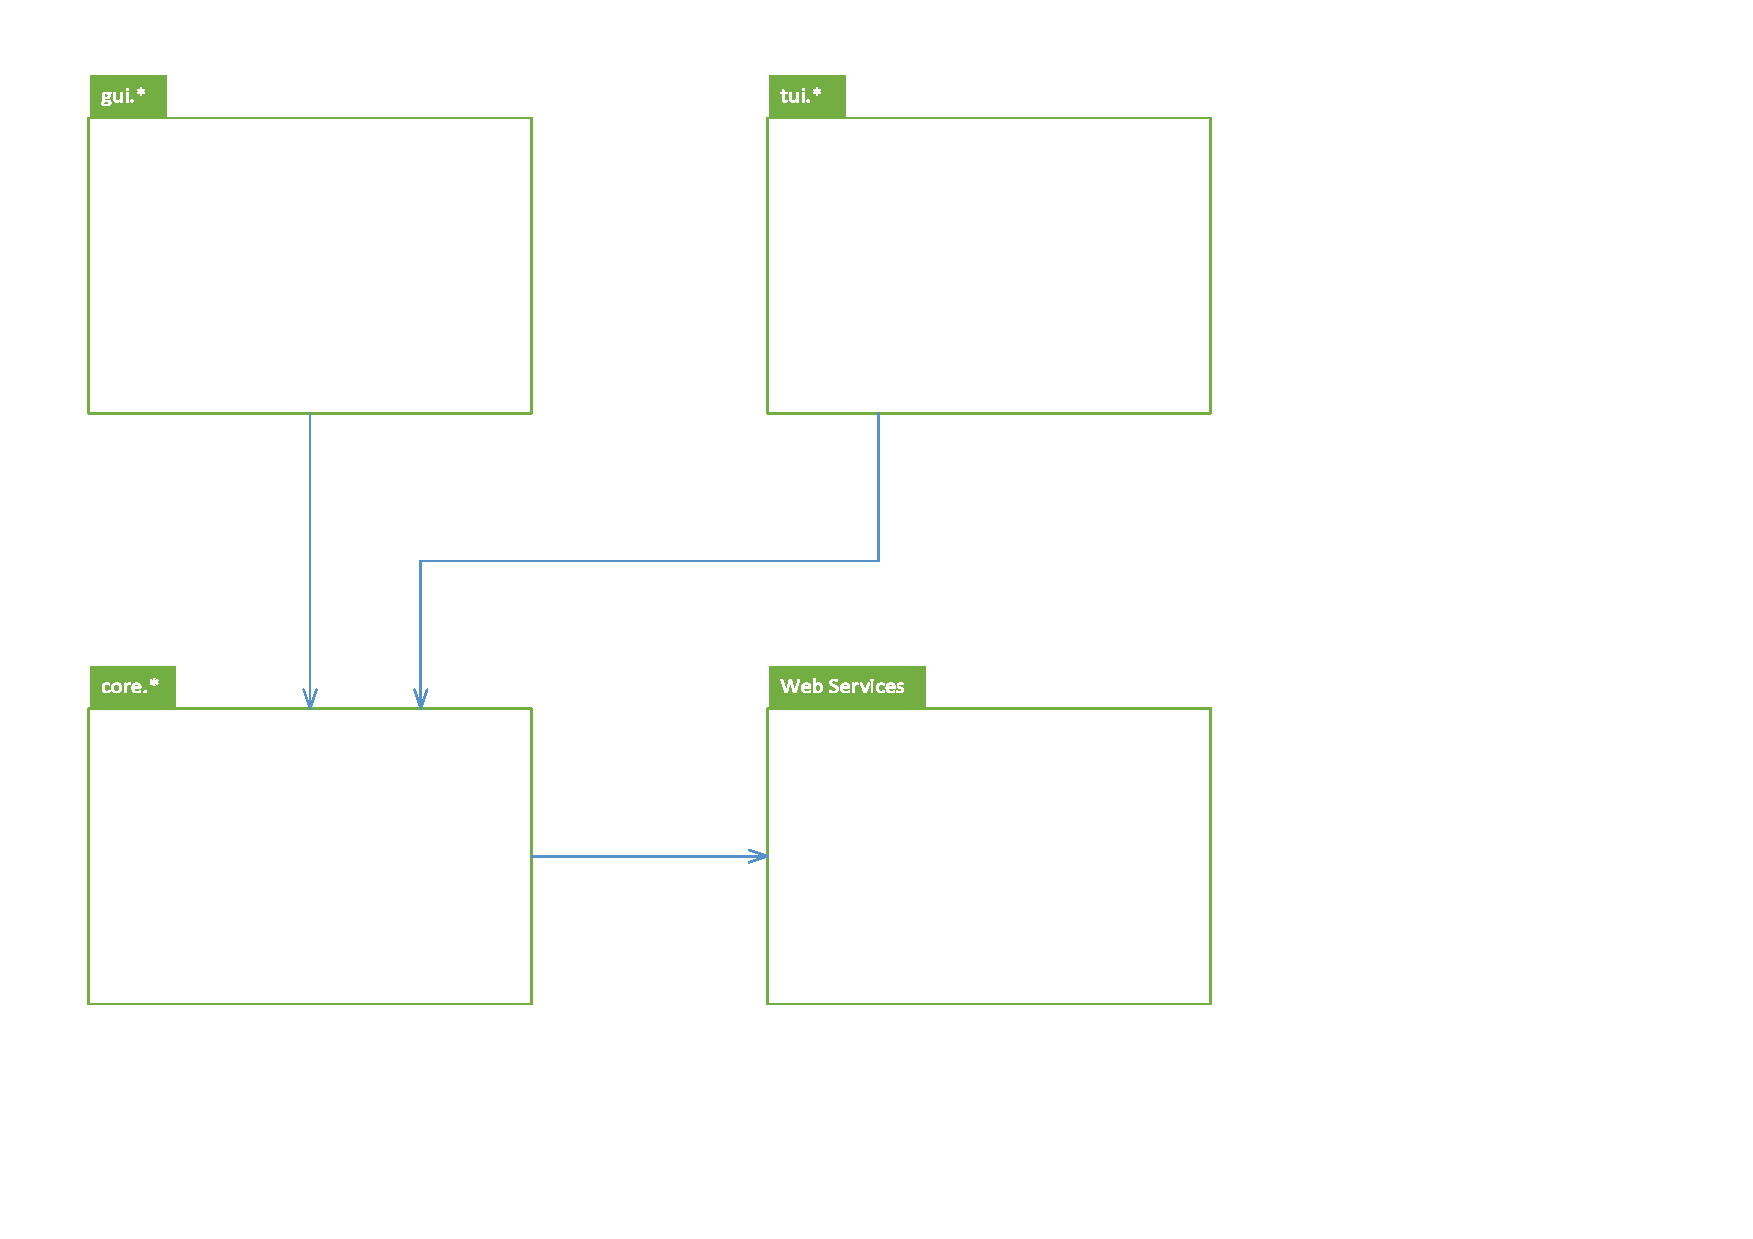
\includegraphics[width=10cm]{Images/ClientOverview}
        \caption{Overview of the packages.}
        \label{fig:ClientOverview}
\end{figure}

For visualization itself JavaFX framework is used. It naturaly enforces
Model-View-Controller architecture.

In the rest of the section the most important packages will be introduced and
described.

\subsection{cz.cuni.mff.ufal.textan.core}

Model classes can be found in this package. It contains mainly client side
representation of object, entity, relation, document etc. (see figure \ref{fig:CorePackage}). Most important class
is \emph{Client} which is used for communication with the webservices. It also
serves as a factory of \emph{ProcessReportPipeline} (see
\ref{sssec:ReportPipeline}). There are also \emph{SynchronizedDataProvider} and
\emph{SynchronizedDocumentProcessor} to provide sychronization for
\emph{IDataProvider} and \emph{IDocumentProcessor} created by CXF.

Subpackages of the \emph{Core} package focus on individual client side tasks,
like displaying graphs and processing report in a pipeline.

\begin{figure}[!htb]
        \centering
        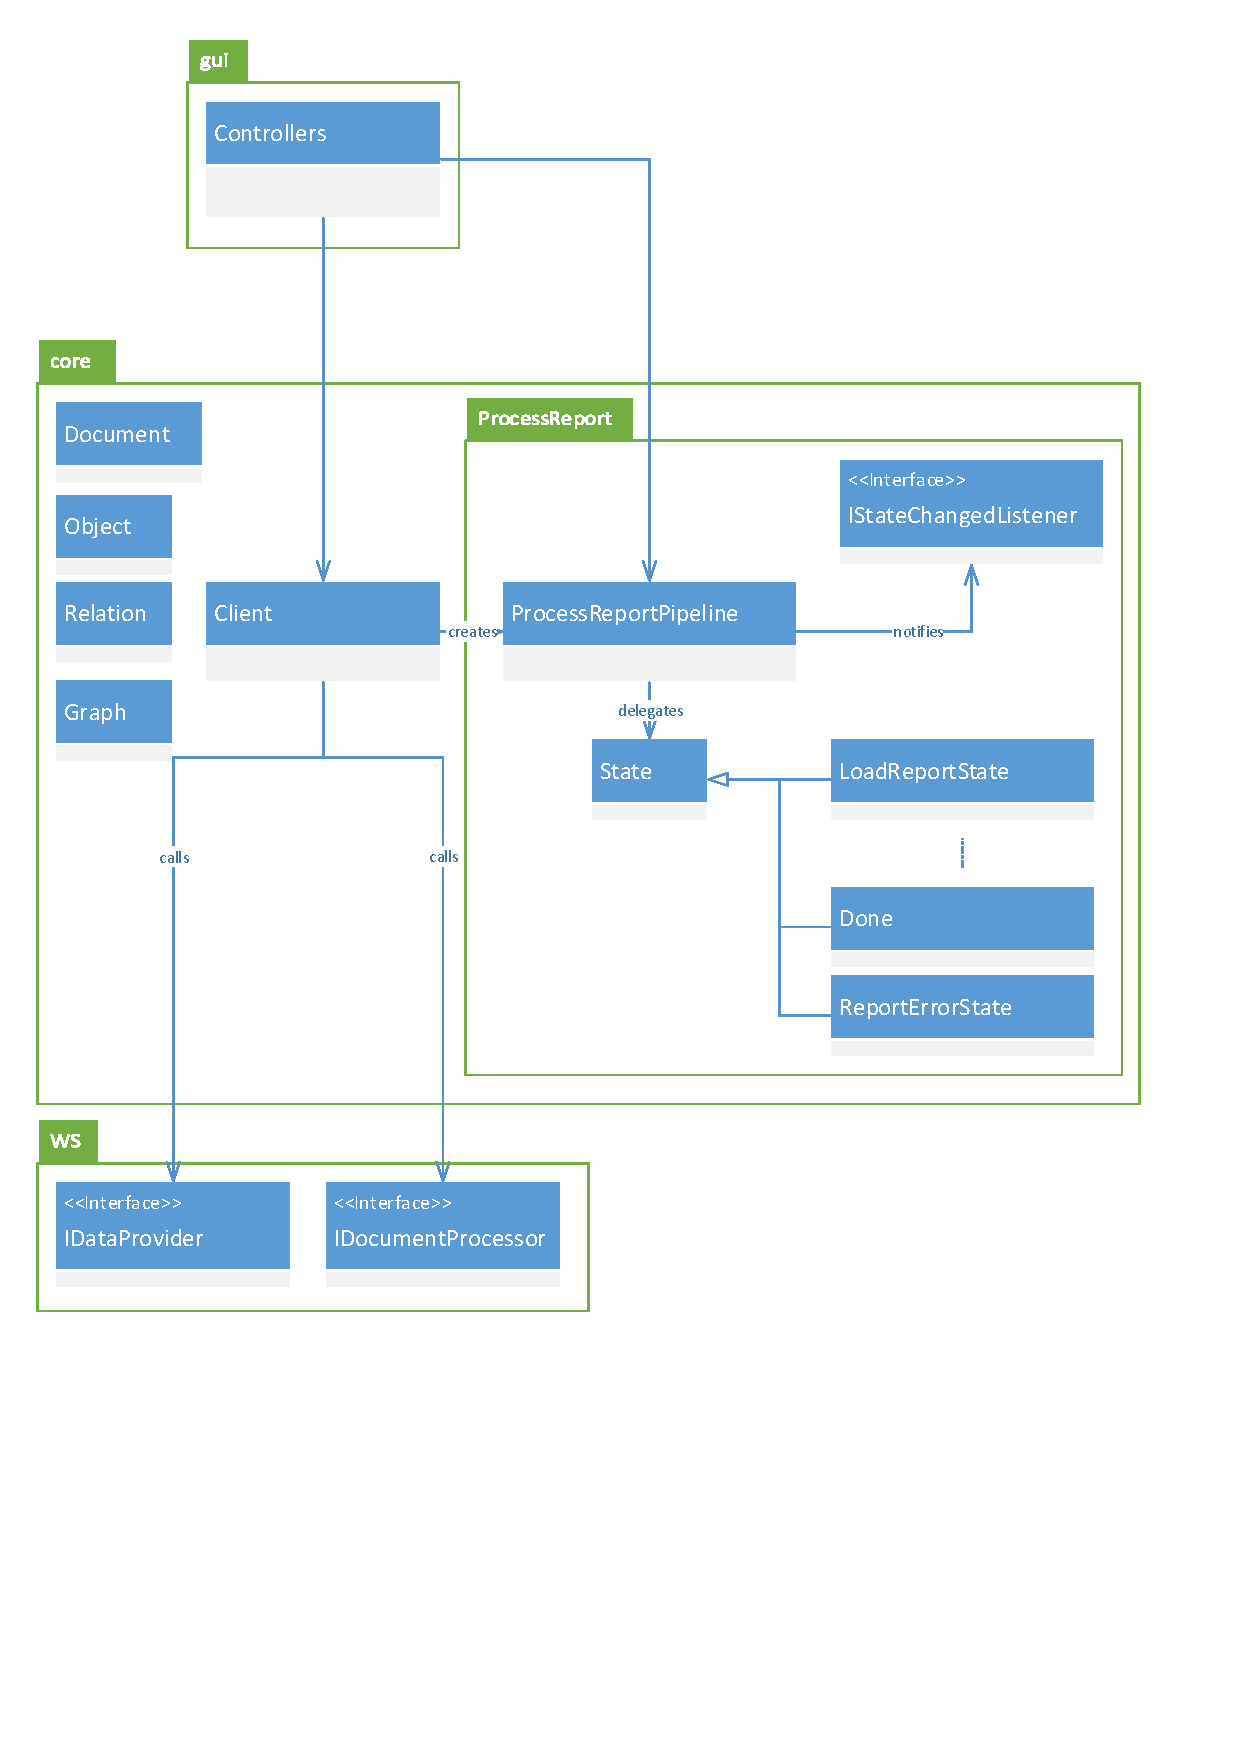
\includegraphics[width=\textwidth]{Images/CorePackage}
        \caption{Overview of the most important features of \emph{core} package.}
        \label{fig:CorePackage}
\end{figure}

\subsubsection{cz.cuni.mff.ufal.textan.core.reportpipeline}
\label{sssec:ReportPipeline}

This package contains classes necessary for report processing (see figure
\ref{fig:CorePackage}). Most importantly there is class
\emph{ProcessReportPipeline} that holds information about processing one report.
The pipeline/wizard approach was chosen because the amount of choices and
required tasks would be overhelming to users if they were all provided at once.
Virtually all methods of the pipeline object are delegated to its \emph{State}
(see figure \ref{fig:Pipeline}). Descendants of the class \emph{State} are
singletons. They contain most of the pipeline processing logic and control to
which state the pipeline should go next. When this happens, each registered
\emph{IStateChangedListener} is notified.

\begin{figure}[!htb]
        \centering
        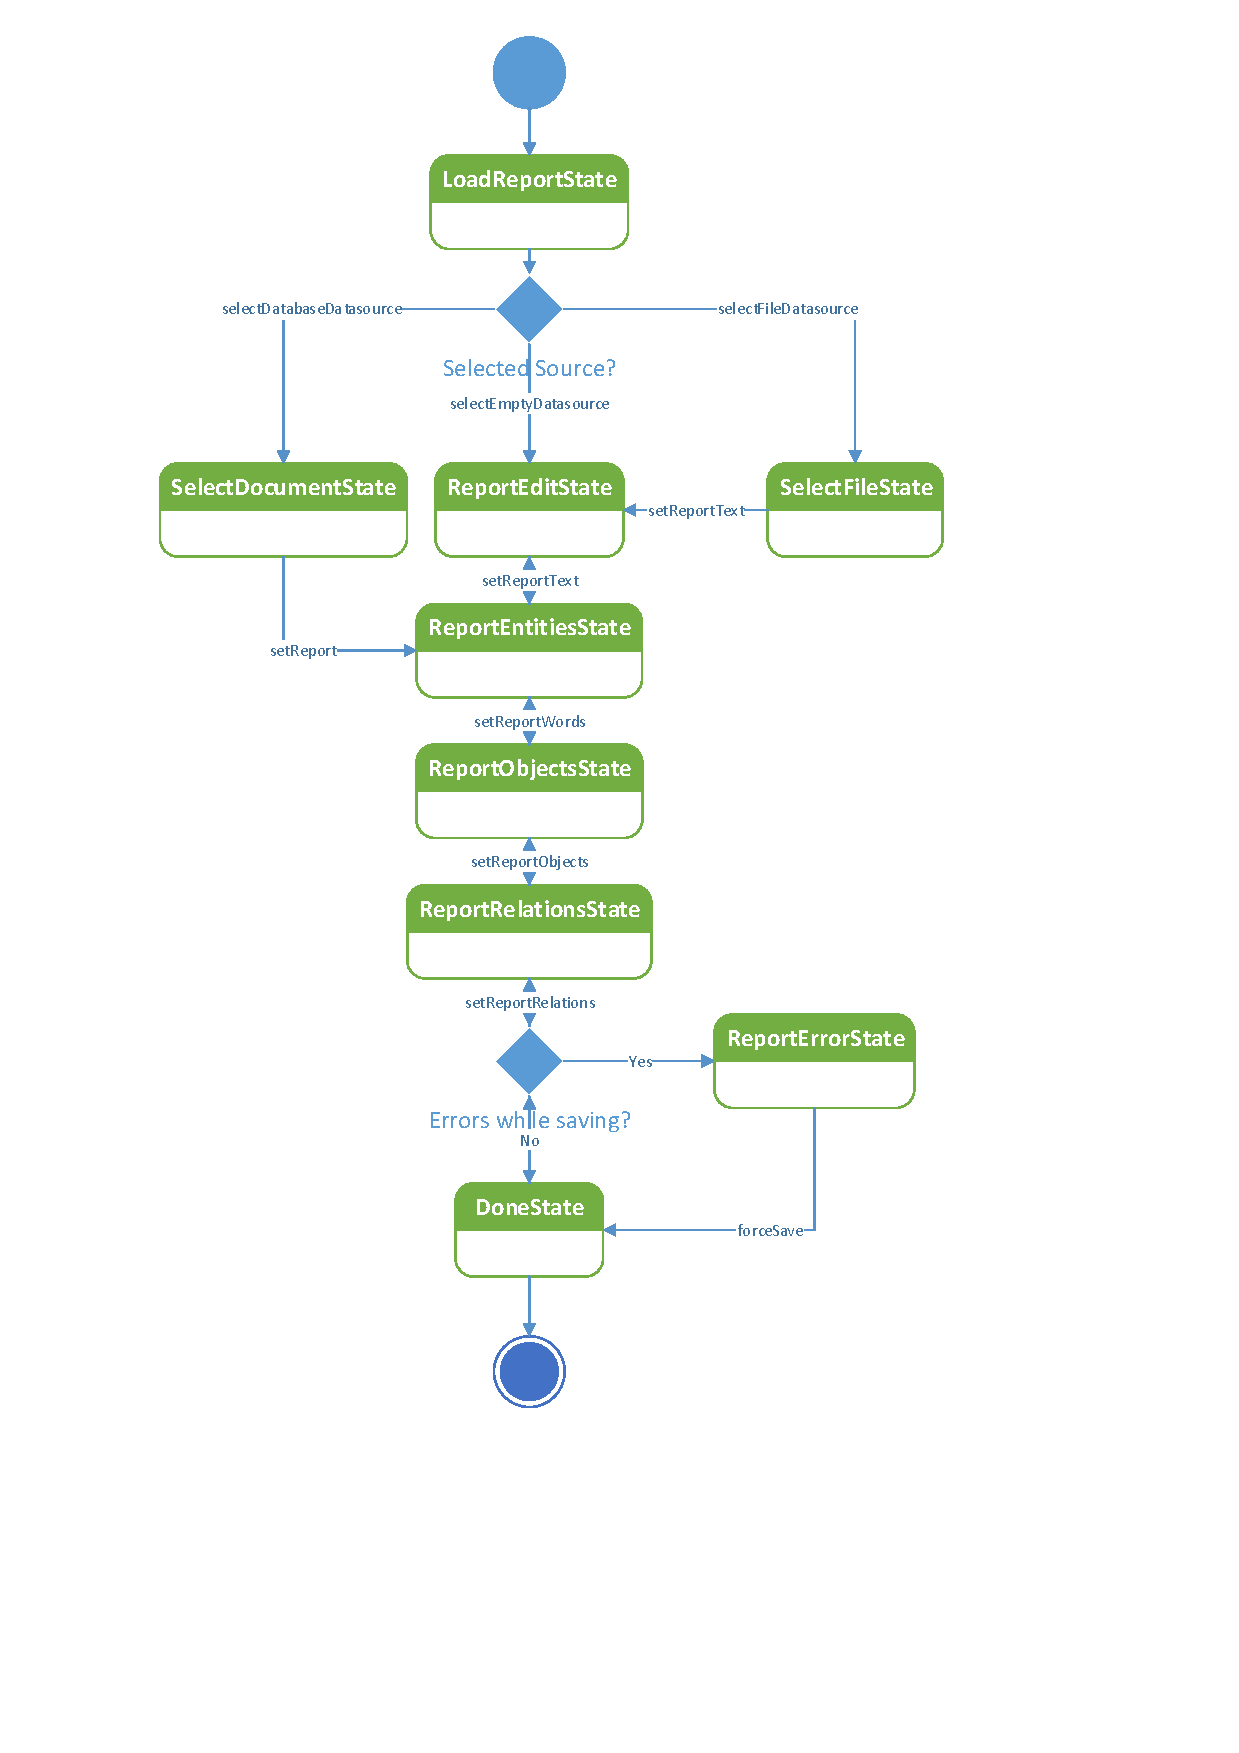
\includegraphics[height=16cm]{Images/Pipeline}
        \caption{Pipeline state machine.}
        \label{fig:Pipeline}
\end{figure}

\subsubsection{cz.cuni.mff.ufal.textan.core.reportpipeline.load}

This package contains classes needed for importing report texts from extenal
files. There is \emph{IImport} interface that provides methods for extracting
text from an array of bytes. Custom implementations of \emph{IImporter} need
to be registered to class \emph{ImportManager} to be selectable by users. The
rest of the package is a few classes providing import of text files in most
common encodings.

\subsubsection{cz.cuni.mff.ufal.textan.core.graph}

This package contains several classes related to creating graphs. They handle
mostly graph filtering which is done solely on client side. See figure
\ref{fig:Graph}.

\begin{figure}[!htb]
        \centering
        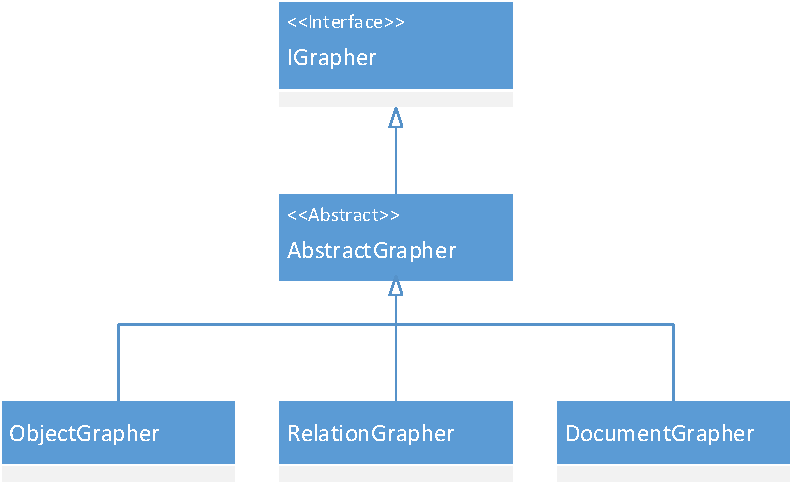
\includegraphics[width=\textwidth]{Images/Graph}
        \caption{Overview of the \emph{graph} package.}
        \label{fig:Graph}
\end{figure}

\subsection{cz.cuni.mff.ufal.textan.gui}

This package and its subpackages contain controller classes and several view
components that had to be customized to achieve specific behaviour. A hierarchy
of controllers has been developed, mostly for code reuse (see
\ref{fig:Controllers}). Controllers extensively use \emph{core} package.

\begin{figure}[!htb]
        \centering
        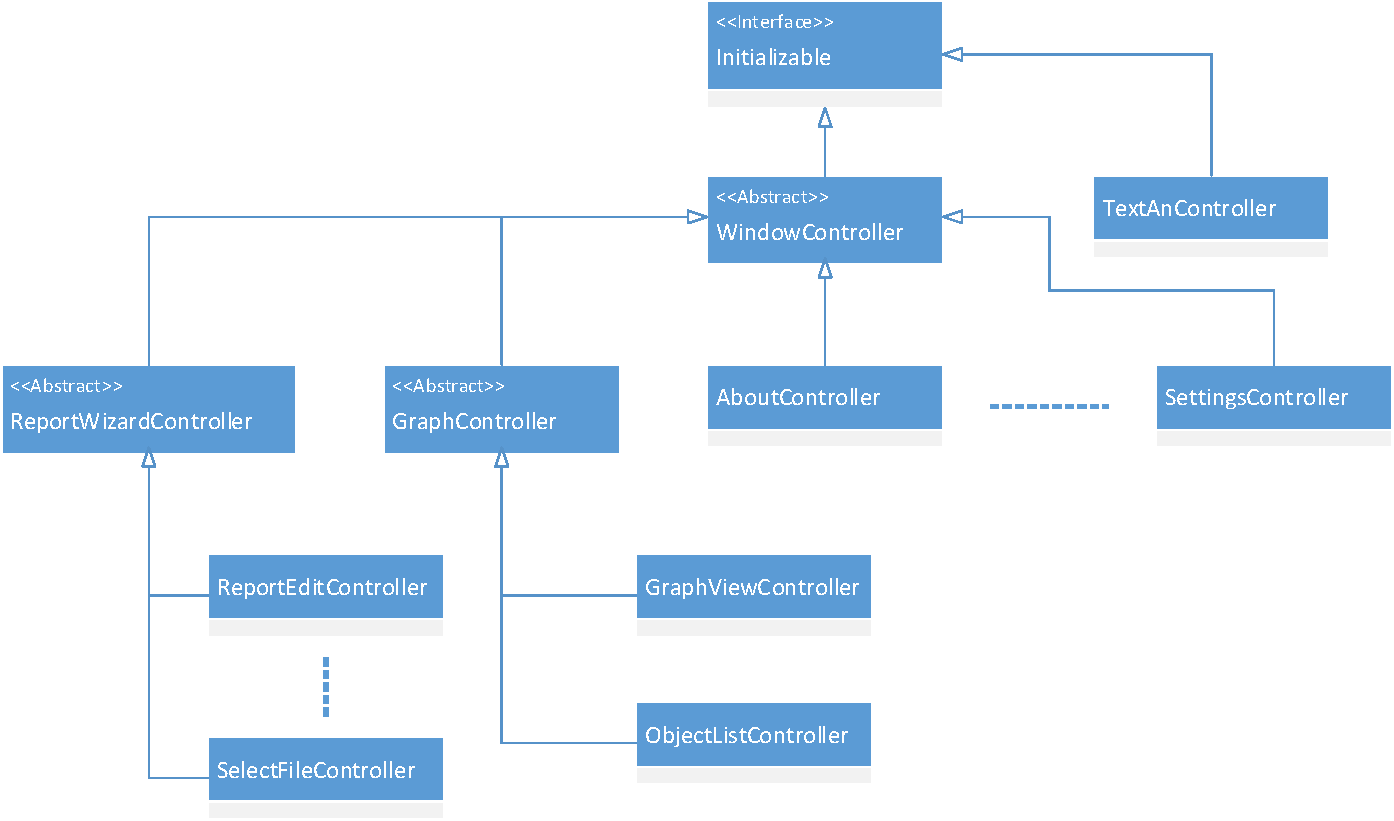
\includegraphics[width=\textwidth]{Images/Controllers}
        \caption{Overview of the controllers hierarchy.}
        \label{fig:Controllers}
\end{figure}

Resources from this package and its subpackages contains descriptions of views
(*.fxml files), styles (*.css files) and localization (*.properties files).

\begin{figure}[!htb]
        \centering
        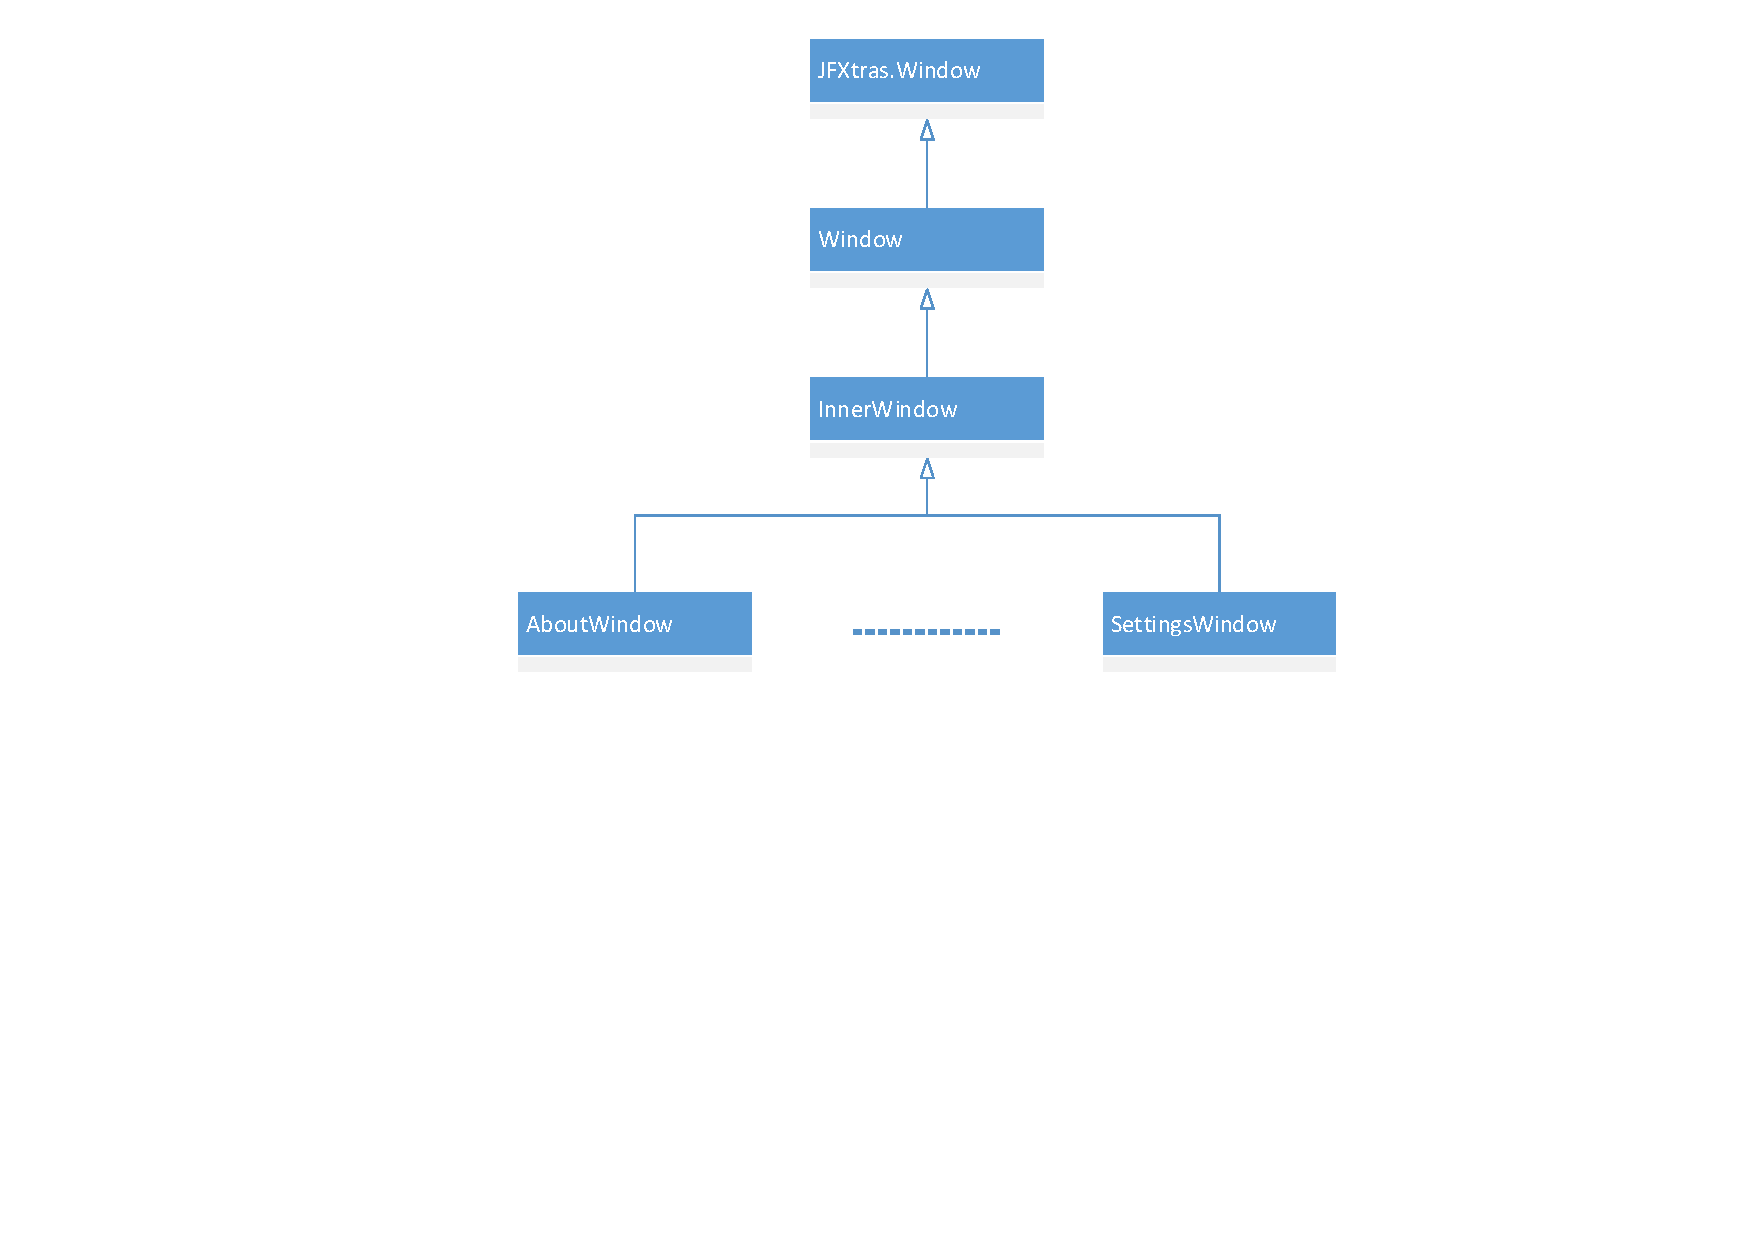
\includegraphics[width=\textwidth]{Images/Windows}
        \caption{Overview of the windows hierarchy.}
        \label{fig:Windows}
\end{figure}

\subsection{cz.cuni.mff.ufal.textan.gui.graph}

This package contains controllers for objects and graph views. The most
interesting class is \emph{GraphView} which embeds JUNG Swing graph into JavaFX
and inserts content of \emph{cz.cuni.mff.udal.textan.core.Graph} to JUNG graph.
Also handles hypergraph conversions if needed for which it uses auxiliary
classes \emph{DummyRelation} and \emph{RelationObject}.

Its only subpackage \emph{string} contains only class \emph{Handler}. It is a
workaround that copes with inability of JavaFX to load css style sheets from
\emph{String} which is needed for \emph{GraphViewController} to generate styles
for coloring filter list checkboxes. For that reason custom url schema "string"
has been created and \emph{Handler} resolves it with strings registered to it.

\subsection{Used Libraries}
\label{ssec:UsedLibraries}

\comment[Adam]{Adam}{Find a suitable place for this section and refactor it.}

\paragraph{ControlsFX\footnote{\url{http://fxexperience.com/controlsfx/}}}
ControlsFX is a Java8 open source library aiming at enhancing the programming
experience with standard JavaFX. It provides wide selection of new and improved
components to make everyday use of JavaFX even easier. \textan{} uses it mainly
for its high quality and user-friendly standard dialogs which are
incomprehensibly and sorely missing in JavaFX.

\paragraph{JCommander\footnote{\url{http://jcommander.org/}}}
JCommander is a very small Java framework that makes it trivial to parse command
line parameters. It was chosen because of easy to used annotaion API and no
external dependencies.

\paragraph{JUNG\footnote{\url{http://jung.sourceforge.net/}}}
JUNG (Java Universal Network/Graph Framework) is older Java library for
displaying graphs, still widely used in Java world, well documented and easily
extensible. Sadly, it does not support JavaFX, but only older Java GUI framework
SWING. Fortunately, thanks to new JavaFX8 SwingNode enabling usage of SWING
components in JavaFX scenes it was possible to seaminglessly integrate JUNG into
JavaFX \textan{} Client.

\paragraph{JFXtras\footnote{\url{http://jfxtras.org/}}}
JFXtras is another JavaFX8 enhancing project. \textan{} Client uses it mostly
for its window management capabilities enabling extensible use of inner windows
embedded into the main window. Another used component is BigDecimalField which
brings common Spinner component into JavaFX.

\paragraph{PretopoLib\footnote{\url{http://pretopolib.complexica.net/}}}
Although JUNG is mature and well thought library, it lacks one important feature
out-of-the-box: displaying hypergraphs. For this reason JUNG graph rendering
part of PretopoLib is used. PretopoLib is a library mainly focusing on
pretopology and graph displaying is rather byproduct. However it fully meets our
requirements and its author kindly provided us the sources so we could fix one
inconvenient detail.